\documentclass[nochap]{apuntes}

\title{Sistemas informáticos - práctica 3}
\author{Guillermo Julián, Víctor de Juan}
\date{Noviembre- 2014}

\begin{document}

\pagestyle{plain}
\maketitle

\tableofcontents
\newpage

\section{Diseño de la base de datos}
\subsection{Entidad - relación}
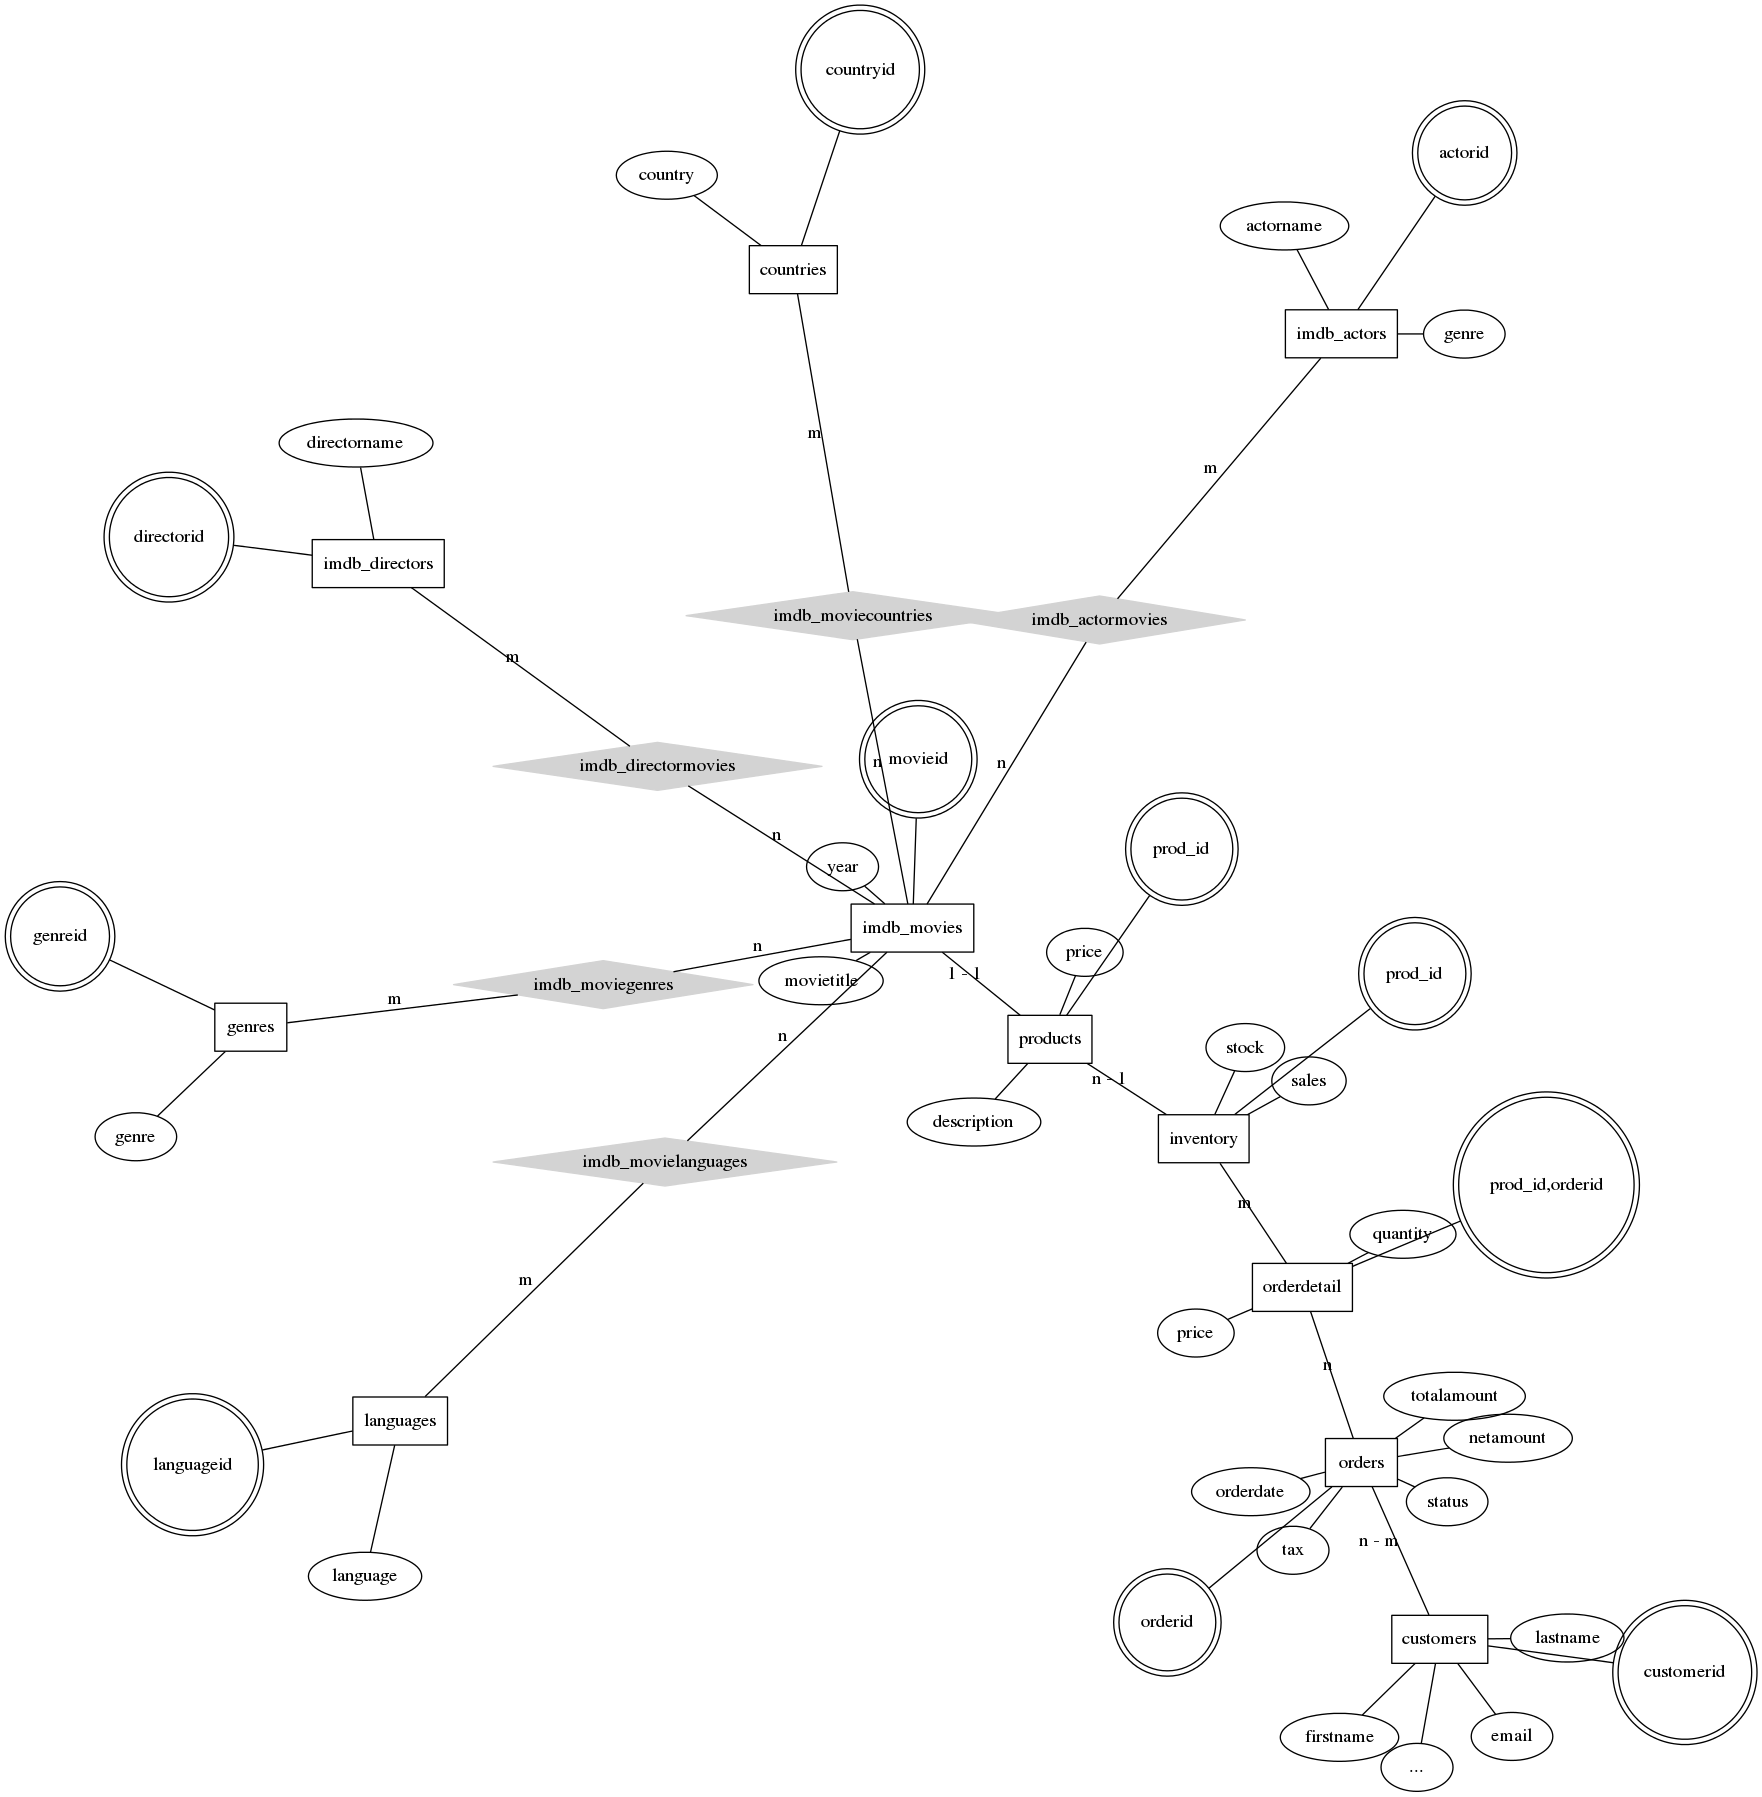
\includegraphics[scale=0.2]{ER.png}

\subsection{Modificaciones sobre la base de datos}

Las modificacinoes en la base de datos se encuentran en el fichero \textit{actualizar.sql} como pedía en enunciado.


Al principio se encuentran las \textit{constraint} necesarias, como claves foráneas. Además, hemos realizado otras las siguientes modificaciones:

\begin{itemize}

\item La clave primaria de orderdetail: Hemos eliminado los ducplicados en orderdetail, ya que la clave primaria  tiene que ser (prod\_id,orderid) ya que es una tabla de la relación $n-m$ de orders con products. 

\item Hemos tenido que insertar algunas filas en inventory para que los datos fueran consistentes y se cumplieran las restricciones de la clave foránea de orderdetail con inventory.

\item Hemos añadido un \textit{UNIQUE} al email de customers para asegurarnos que podemos hacer consultas de búsquedas de clientes por el email. Además, le hemos puesto un índice para optimizar las consultas de búsqueda en el login.

\item Hemos añadido una columna a la tabla \textit{imdb\_movies} llamada \textit{url\_to\_img} para mejorar la interfaz. Hay un archivo llamado \textit{images.sql} que inserta en la tabla las url de las imágenes (que hemos obtenido de imdb.com con un script en python). Las películas de las que no hayamos encontrado imagen en imdb.com tendrán una por defecto.

\item Hemos separado también las tablas de género (de película), país e idiomas. 

\item Por último, hay que actualizar el valor de las sequencias de las tablas en las que insertamos cuya clave primaria es un serial, es decir, en \textit{orders} y en \textit{customers}. Para ello hemos creado un procedimieto llamado \textit{alter\_sequences()}.
\end{itemize}



\section{Consultas, procedimientos almacenados y triggers}
\subsection{setItemPrice}
El proceso para actualizar los precios se encuentra en un fichero aparte. Realizamos con un update y una tabla auxiliar.
\subsection{setOrderAmount,getTopVentas}
Se encuentran en el fichero \textit{actualizar.sql} y no hay nada digno de ser mencionado.
\subsection{getTopMonth}
Hemos escrito este procedmiento en leguaje \textit{sql} y no en \textit{plpgsql} porque nos parecía interesate invstigar otros lenguajes de procedimientos almacenados y en este caso en concreto, en \textit{sql} es muy fácil ejecutar sentencias.

\subsection{updOrders}
Como no hemos implementado el carrito en la base de datos, no hemos implementado este trigger, ya que no es necesario para nuestra implementación. 

\subsection{updInventory}
Este trigger no se podía lanzar antes de la inserción en orders, ya que requiere que se haya insertado previamente las correspondientes filas en \textit{orderdetail}, y no es posible insertar en \textit{orderdetail} una fila con un \textit{orderid} que no referencie a ningún \textit{orderid}, dado que todavía no se ha insertado.

Asíque, el  procedimiento seguido es el siguiente:
\begin{itemize}
\item 1) Insertamos en \textit{orders}, con el estado a NULL.
\item 2) Insertamos las filas correspondientes en \textit{orderdetail}.
\item 3) Actualizamos el valor del estado de orders y esto es lo que lanza el trigger.
\end{itemize}

Nos encontramos el problema de cómo asegurarnos que no se vendían más películas de las que hubiera en stock. Pensamos que es una solución mejor acercar esta comprobación al lado del cliente. Si no voy a poder comprar una película, ¿para qué dejar añadirla al carrito?. Hemos añadido a la funcionalidad del carrito la comprobación del stock, de tal manera que no puedan llegar peticiones de compra de más productos de los que tenemos. 

Como esto se controla en JS desde el lado del cliente, es posible que hubiera problemas de concurrencia, que esto lo solucionaremos en la siguiente práctica, como nos comentaste.


\section{Modificaciones sobre el HTML, JS y PHP}
En general no ha habido que realizar grandes cambios, debido a que intentamos ser lo más modulares posibles. Además, como nuestro JS trabaja con array's que le pide al servidor, entonces con cambiar el lado del servidor ha sido suficiente.

Lo que sí hemos cambiado es añadir al carrito un campo más al array de compras para controlar el stock como hemos mencionado anteriormente.

\subsection{Historial y películas}
Sólo hemos tenido que cambiar el lado del servidor (como ya hemos mencionado) ya que el lado del cliente utiliza array's que obtiene del servidor.


\subsection{Registrarse y Login}

Solo ha sido necesario cambiar el fichero \textit{/php/login\_register.php} en el que se realizan las comprobaciones de login y registrarse. Utilizamos un \textit{PDO} para poder preparar las consultas, ya que siempre serán del mismo tipo, cambiando algún argumento, para lo que utilizamos el método \textit{bindParams}.



\end{document}